% ============================================================
%  Capítulo 3 — Arquitetura do Sistema
% ============================================================
\chapter{ARQUITETURA DO SISTEMA}
\label{cap:arquitetura}

\section{Visão geral do pipeline}
\label{sec:pipeline}

O sistema é composto por quatro camadas sequenciais: instrumentação dos motores
JavaScript, captura de chamadas de API por extensão de navegador, coleta
automatizada por crawlers e pós-processamento para produção do dataset
rotulado. A Figura~\ref{fig:pipeline} apresenta o pipeline completo.

\begin{figure}[htb]
\centering
\caption{Pipeline de instrumentação, coleta e processamento cross-engine}
\label{fig:pipeline}
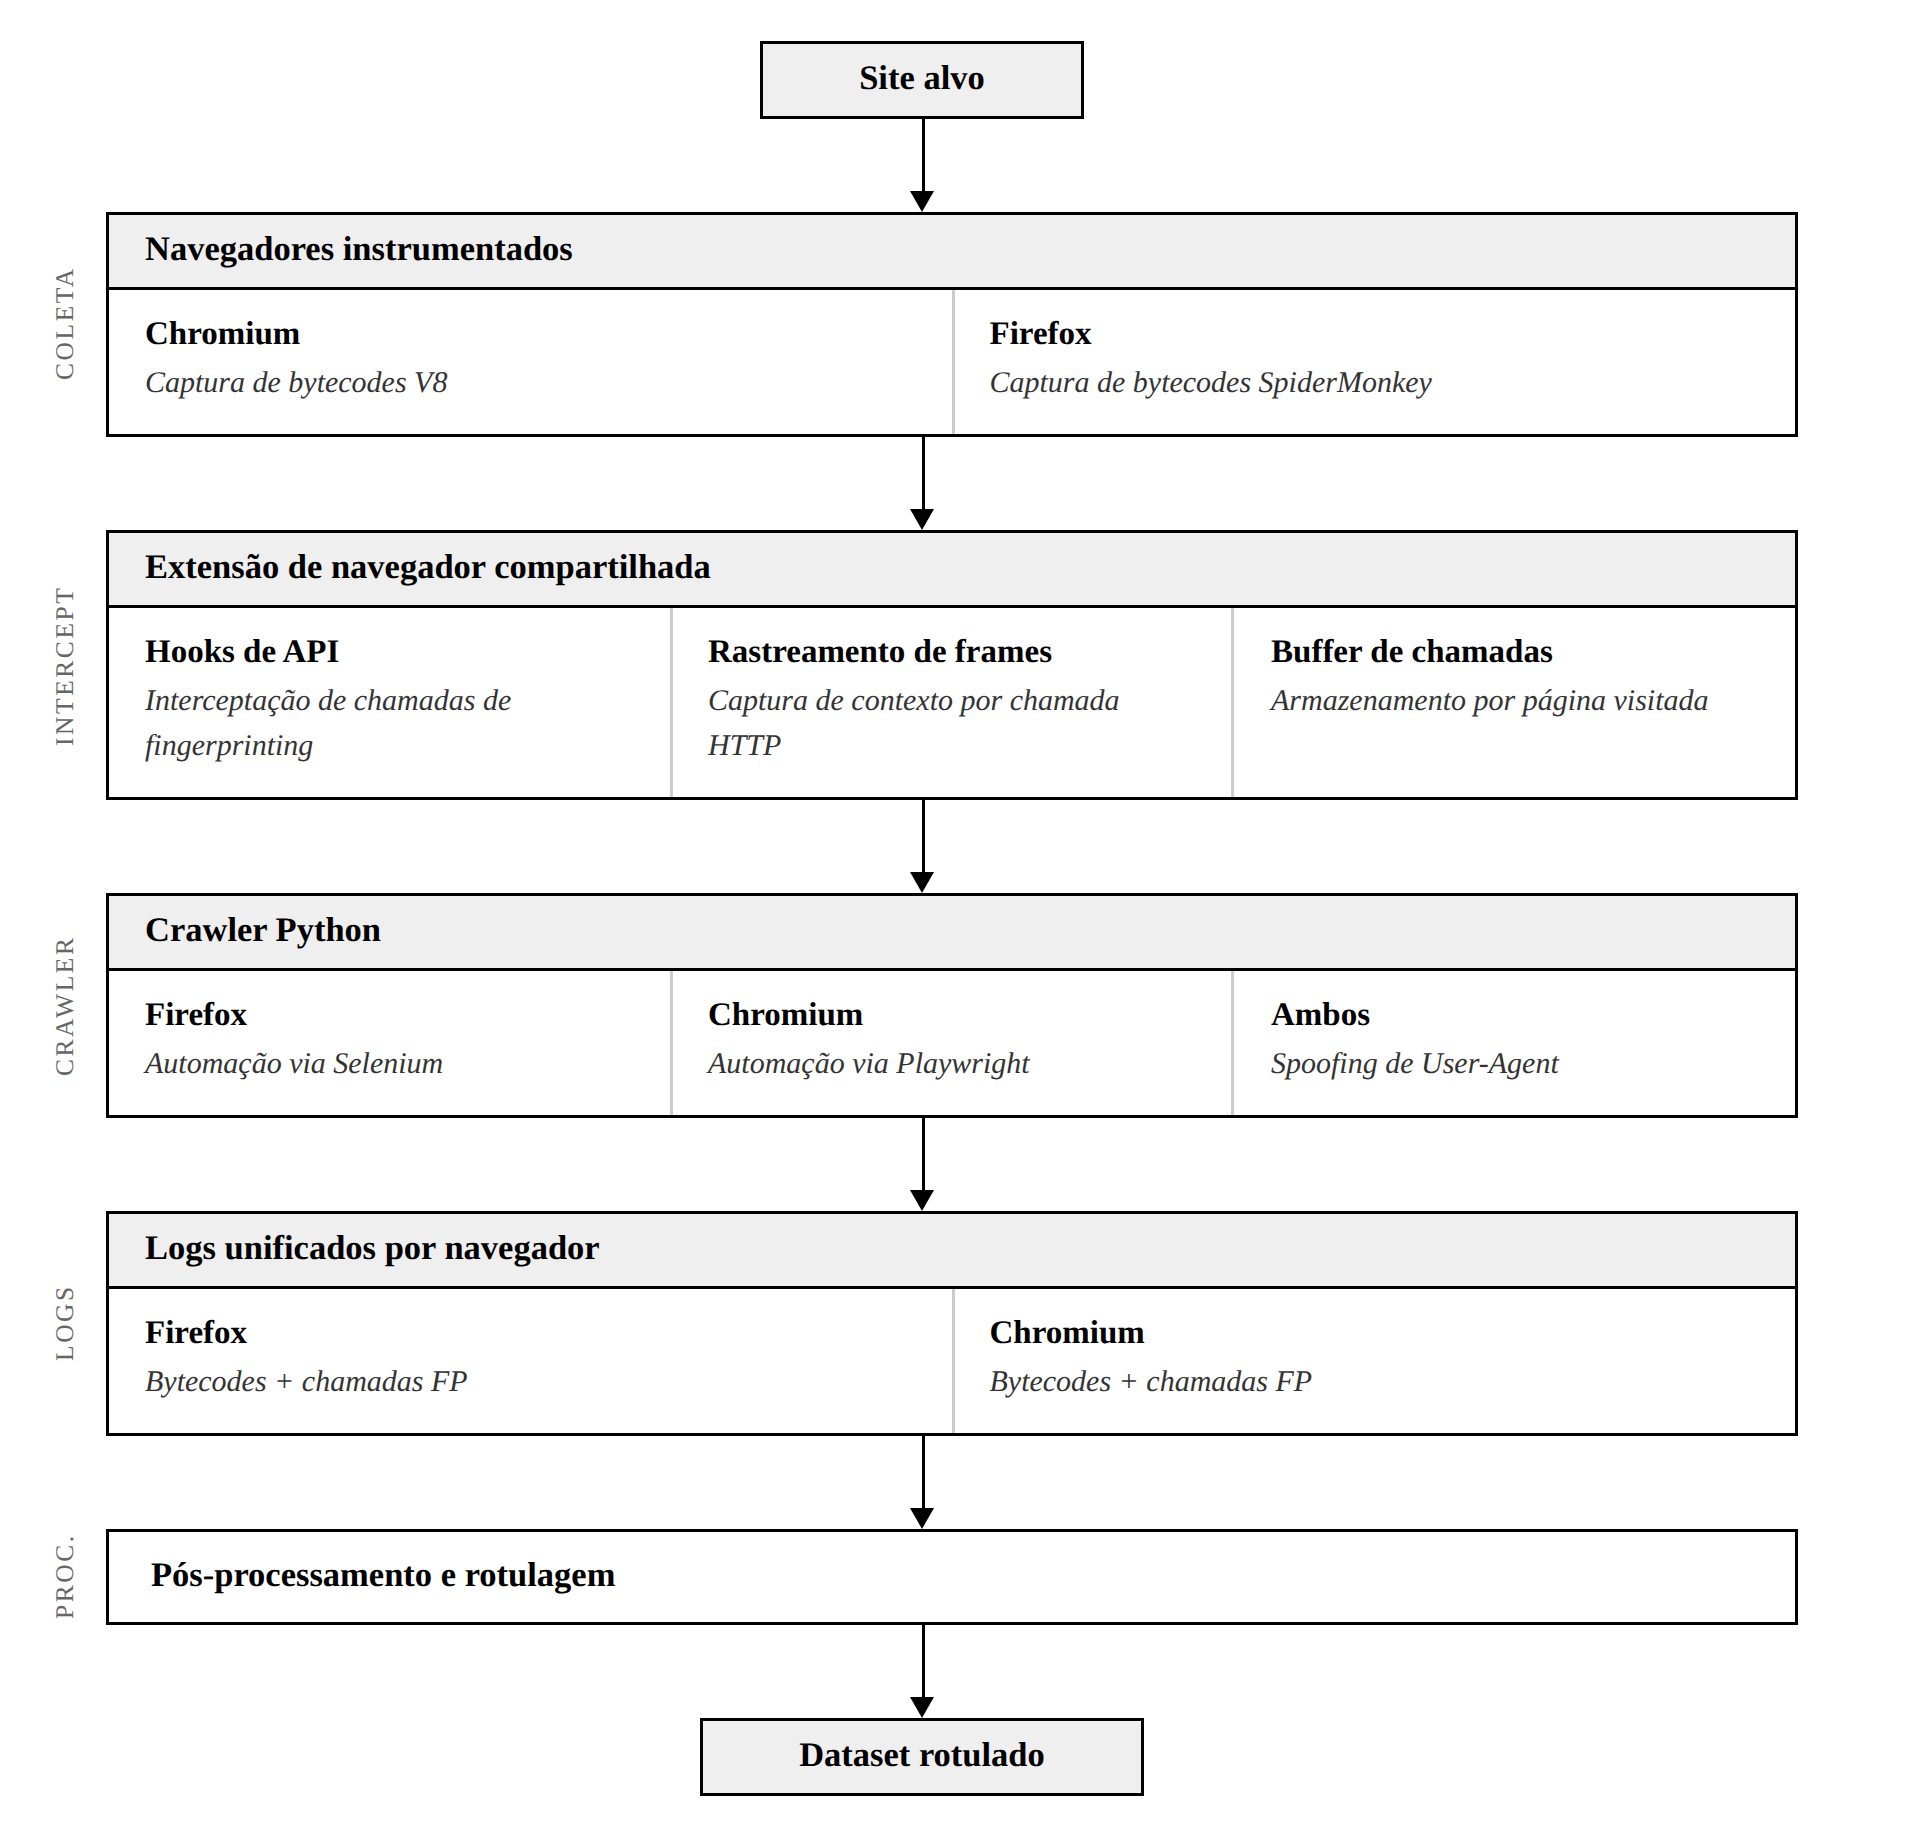
\includegraphics[width=\textwidth]{pipeline}
\fonte{Elaborada pelo autor.}
\end{figure}

O formato JSONL de bytecodes é unificado entre os dois navegadores, com os campos
\texttt{browser}, \texttt{injected\_id}, \texttt{script\_url}, \texttt{script\_id},
\texttt{function\_name} e \texttt{bytecodes} presentes em ambos. O campo
\texttt{injected\_id} possui semântica distinta nos dois motores e é descrito nas
seções seguintes.

%, , , , , , , , , , , , , , , , , , , --
\section{Instrumentação do V8}
\label{sec:v8}

A instrumentação é inserida no interpretador Ignition, invocada ao término
da compilação de cada função JavaScript. Para cada função, um identificador
estável é computado via hash FNV-1a de 64 bits sobre a combinação de URL do
script e posições de início/fim no código-fonte, garantindo reprodutibilidade
entre sessões. Funções sem script associado (built-ins e módulos internos) são
descartadas. Cada registro é emitido para o fluxo de erro padrão com o prefixo
\texttt{[V8Log]}, contendo identificador, URL, posições e sequência de bytecodes.
O código completo de instrumentação está no Apêndice~\ref{ap:instrumentacao}.

%, , , , , , , , , , , , , , , , , , , --
\section{Instrumentação do SpiderMonkey e injeção de ID para funções anônimas}
\label{sec:sm}

\subsection{Formato de emissão}
\label{sub:sm-formato}

A instrumentação do SpiderMonkey emite um bloco de texto por função compilada,
identificado pelo prefixo \texttt{[SpiderMonkey Log]}, com URL do script, nome da
função e sequência de bytecodes. O formato usa múltiplas linhas por registro,
ao contrário do JSON de linha única do V8. Um exemplo completo está no
Apêndice~\ref{ap:crawler-ext}.

\subsection{O problema das funções anônimas}
\label{sub:sm-anon}

Em bundles JavaScript minificados, a grande maioria das funções não possui
nome: \texttt{Function name} aparece como string vazia no log do SpiderMonkey. Sem
nome, não é possível ligar o registro de bytecodes a uma chamada de API capturada
pela extensão, o \texttt{Error.stack} expõe o nome da função chamadora, e uma
string vazia produz colisões massivas no join.

A solução implementada neste trabalho é a \textbf{injeção de identificador único
como \texttt{displayName}}: no código-fonte do SpiderMonkey, funções anônimas
recebem um nome sintético no formato \texttt{anon\_injected\_ID} no momento da
compilação, onde \texttt{ID} é um hash de 64 bits baseado em atributos da função
(URL do script e índice interno). Esse nome é armazenado como \texttt{displayName}
da função, que o motor do JavaScript propaga automaticamente para
\texttt{Error.stack} quando a função aparece na pilha de chamadas.

O efeito prático é que a extensão de navegador, ao capturar um \texttt{Error.stack}
durante uma chamada a \texttt{canvas.toDataURL}, enxerga o nome
\texttt{anon\_injected\_ID} na pilha, mesmo que a função não tenha nome no
código-fonte original, e o registra em \texttt{funcName}. O parser do
crawler encontra o registro de bytecodes com exatamente o mesmo
\texttt{function\_name}, e o join ocorre sem perda de dados.

Essa abordagem eliminou a perda de dados que afetava aproximadamente 38\% das
funções anônimas na versão anterior do pipeline, que tentava identificar funções
por posição no script.

\subsection{Parser do log SpiderMonkey}
\label{sub:sm-parser}

O crawler Firefox processa o log do geckodriver ao final de cada batch de
sites: identifica os blocos \texttt{[SpiderMonkey Log]}, descarta URLs internas
do Firefox, deduplica registros entre batches e converte o resultado para o
formato JSONL unificado. Detalhes estão no Apêndice~\ref{ap:instrumentacao}.

%, , , , , , , , , , , , , , , , , , , --
\section{Extensão de navegador: hooking de APIs e captura de pilha multi-frame}
\label{sec:extensao}

\subsection{Arquitetura e hooking de protótipos}
\label{sub:ext-arq}

A extensão compartilhada é uma extensão Manifest V3 carregada por ambos os
navegadores. Seu script de conteúdo é injetado antes de qualquer script do
site, garantindo que os hooks estejam ativos desde o início do carregamento da
página. A interceptação é feita por substituição de métodos nos protótipos das
APIs alvo; propriedades somente leitura são redefinidas com preservação dos
valores originais. Os detalhes de implementação estão no
Apêndice~\ref{ap:crawler-ext}.

As 32 APIs monitoradas estão listadas na Tabela~\ref{tab:apis}.

\begin{table}[htb]
\centering
\caption{APIs interceptadas pela extensão de navegador}
\label{tab:apis}
\begin{tabularx}{\linewidth}{l>{\raggedright\arraybackslash}X}
\toprule
\textbf{Categoria} & \textbf{Métodos / Propriedades interceptados} \\
\midrule
Canvas          & \texttt{toDataURL}, \texttt{getImageData}, \texttt{fillText}, \texttt{measureText}, \texttt{font} (setter), \texttt{save}, \texttt{restore} \\
OffscreenCanvas & \texttt{fillText}, \texttt{measureText}, \texttt{font} (setter) \\
Áudio           & \texttt{createOscillator}, \texttt{createDynamicsCompressor}, \texttt{startRendering}, \texttt{connect}, \texttt{copyFromChannel}, \texttt{getChannelData} \\
WebGL~1         & \texttt{getParameter}, \texttt{getSupportedExtensions} \\
WebGL~2         & \texttt{getParameter} \\
Tela            & \texttt{colorDepth}, \texttt{pixelDepth}, \texttt{width}, \texttt{height}, \texttt{availWidth} \\
Navigator       & \texttt{hardwareConcurrency}, \texttt{languages}, \texttt{platform}, \texttt{deviceMemory}, \texttt{maxTouchPoints} \\
WebRTC          & \texttt{createOffer}, \texttt{createDataChannel}, \texttt{setLocalDescription} \\
\bottomrule
\end{tabularx}
\fonte{Elaborada pelo autor.}
\end{table}

\subsection{Captura de pilha multi-frame}
\label{sub:ext-stack}

Para cada chamada de API interceptada, a extensão captura a pilha de chamadas
completa e registra todos os frames HTTP presentes, não apenas o chamador
imediato. Essa estratégia é necessária para que o pós-processador atribua
rótulos às funções orquestradoras que delegam chamadas de API para sub-rotinas
internas. Os detalhes de implementação, incluindo o tratamento de diferenças de
formato de stack trace entre V8 e SpiderMonkey, estão no
Apêndice~\ref{ap:crawler-ext}.

%, , , , , , , , , , , , , , , , , , , --
\section{Normalização de propriedades do Firefox}
\label{sec:normalizacao}

Uma condição necessária para o alinhamento cross-engine é que os sites web sirvam
o mesmo bundle JavaScript aos dois navegadores e que as bibliotecas de
fingerprinting executem os mesmos caminhos de código em ambos. Por padrão,
isso não ocorre: o Firefox expõe propriedades exclusivas que essas bibliotecas
detectam para selecionar implementações alternativas, ou para pular
completamente vetores como Canvas.

A extensão, executada em \texttt{document\_start}, realiza as seguintes
normalizações antes que qualquer script do site execute:

\textbf{Adições para simular Chromium:}
\begin{itemize}
  \item \texttt{window.chrome = \{ runtime: \{\} \}}, presente no Chromium,
    ausente no Firefox; a ausência é usada por bibliotecas como FingerprintJS para
    detectar Firefox.
  \item \texttt{navigator.vendor = 'Google Inc.'}, o Firefox retorna string
    vazia; o Chromium retorna \texttt{'Google Inc.'}.
\end{itemize}

\textbf{Remoções de propriedades exclusivas do Firefox:}
\begin{itemize}
  \item \texttt{navigator.buildID, navigator.globalPrivacyControl, navigator.oscpu}, presentes apenas no Firefox; usados como
    indicadores de motor pelo FingerprintJS e similares.
  \item \texttt{window.mozInnerScreenX}, \texttt{window.onmozfullscreenchange},
    \texttt{document.documentElement.style.MozAppearance}, propriedades
    prefixadas \texttt{moz}, detectadas por heurísticas de identificação de motor.
\end{itemize}

Além disso, o User-Agent é configurado no crawler Firefox para o valor
idêntico ao do Chromium~131 (string completa no Apêndice~\ref{ap:crawler-ext}).

O efeito combinado dessas normalizações é que sites que utilizam
\texttt{isFirefox()} ou verificações análogas para desviar o fluxo de coleta de
fingerprints passam a executar o mesmo código nos dois navegadores,
produzindo chamadas de API comparáveis entre sessões. Sem essas normalizações,
sites como os que utilizam FingerprintJS produzem zero chamadas à Canvas API no
Firefox.

%, , , , , , , , , , , , , , , , , , , --
\section{Crawlers}
\label{sec:crawlers}

Os dois crawlers visitam os 10.000 sites-alvo com Firefox e Chromium
instrumentados, emitindo logs no formato JSONL unificado. Ambos simulam
interação humana após o carregamento das páginas para ativar fingerprinting
condicionado a eventos, impõem timeout por site e são idempotentes,
permitindo retomada sem reprocessamento após falhas. Os detalhes de
implementação estão no Apêndice~\ref{ap:crawler-ext}.

%, , , , , , , , , , , , , , , , , , , --
\section{Estratégia de join: bytecodes <---> chamadas de API}
\label{sec:join}

O pós-processador liga cada registro de bytecodes ao conjunto de chamadas de
API observadas na mesma função, produzindo as colunas de rótulo multilabel do
dataset. A estratégia de join varia segundo o motor e o tipo
de função (Tabela~\ref{tab:join}).

\begin{table}[htb]
\centering
\caption{Estratégias de join por motor e tipo de função}
\label{tab:join}
\begin{tabularx}{\linewidth}{llX}
\toprule
\textbf{Motor} & \textbf{Tipo de função} & \textbf{Estratégia} \\
\midrule
Firefox (SM) & Nomeada & Join por nome da função \\
Firefox (SM) & Anônima & Join por nome: ID injetado (\texttt{anon\_injected\_ID}) propaga-se para o call stack \\
Chromium (V8) & Nomeada & Join por (URL do script, nome da função) \\
Chromium (V8) & Anônima & Join por posição: (linha, coluna) convertido a offset de caractere \\
\bottomrule
\end{tabularx}
\fonte{Elaborada pelo autor.}
\end{table}

Para o Chromium, o offset de caractere é determinado a partir de linha e
coluna; o intervalo mais interno é selecionado para resolver sobreposições de
funções aninhadas. As heurísticas de rotulagem multilabel que determinam as
categorias de fingerprinting a partir do padrão de chamadas de API observado
são descritas em detalhe no Capítulo~\ref{cap:dataset}.
